\chapter{Probelmanalyse}

    In dem Laborprojekt soll ein Softcore entwickelt werden der den \textit{RV32I} Befehlssatz implementiert.
    Dieser soll auf einem \textit{FPGA}-Board hochgeladen werden und Programmcode ausführen können.
    Zusätzlich soll durch Simulationstests sowie durch Tests durch Programmcode die Korrektheit
    bewiesen werden.
    Die Aufgabenstellung kann in Soft- und Hardware unterteilt werden.

        \section{Software}
            Aus Softwaresicht wird eine Toolchain benötigt die Programmcode compiliert
            und in ein Dateiformat bringt, welches vom Softcore interpretiert werden kann.
            \\
            Dies wird im folgendem Kapitel \ref{lab:toolchain} behandelt.

        \section{Hardware}\label{lab:hardware}
            Aus Hardwaresicht wird ein \textit{FPGA}-Board benötigt welches eine Möglichkeit bietet
            den in \textit{VHDL} modellierten Softcore auf das \textit{FPGA}-Board sowie Programmcode
            in den Softcore zu laden.
            \\\\
            Die Wahl fällt auf das \textit{FPGA}-Board \textit{TEI0003 TRM} von \textit{Trenz Electronic}.
            Herz des Boards ist der \textit{Cyclone 10LP 10CL025 FPGA SoC} von Intel der an einem $12 Mhz$
            Oszillator angeschlossen ist. 
            Als Speicher stehen 66 \textit{M9K}-Blöcke \cite{intel-cyc10lp-io-datasheet}[2.1 Tabelle 2] mit jeweils 8.192 Bit
            \cite{intel-cyc10lp-io-datasheet}[2.2] ($66*8192/8 = 67584B$) des \textit{Cyclone 10LP} sowie $8 MB$ des \textit{TEI0003-02} zu Verfügung.
            Abbildung \ref{fig:fpga_schematic} zeigt den schematischen Aufbau des \textit{TEI0003 TRM}.
            \begin{figure}[H]
                \centering
                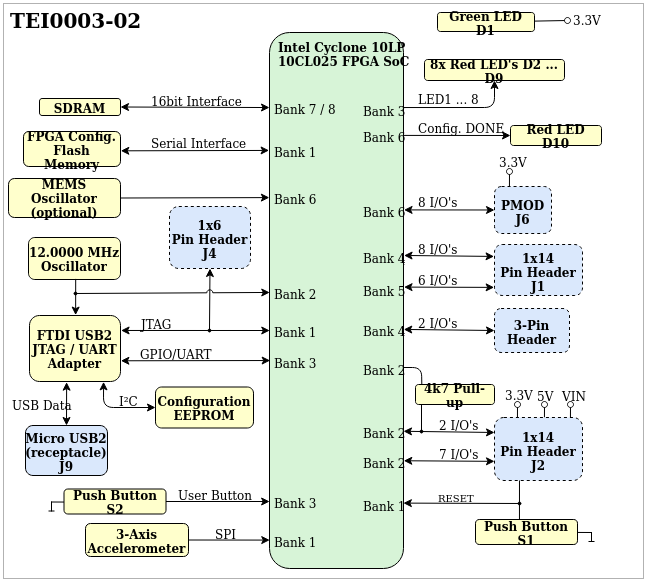
\includegraphics[scale=0.5]{img/fpga_board_schematic.png}
                \caption[Schaubild des TEI0003 TRM FPGA-Board]{Schaubild des TEI0003 TRM FPGA-Board \cite{terz} }
                \label{fig:fpga_schematic}
            \end{figure}

            \begin{figure}[H]
                \centering
                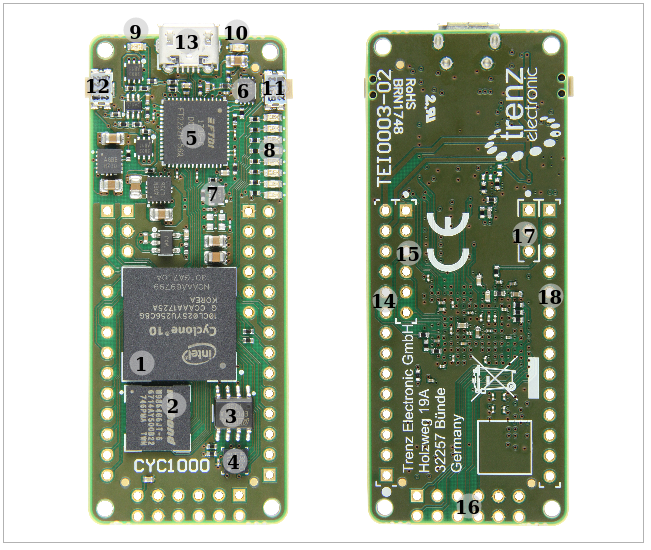
\includegraphics[scale=0.5]{img/fpga_board_layout.png}
                \caption[Platine des TEI0003 TRM FPGA-Board]{Platine des TEI0003 TRM FPGA-Board \cite{terz} }
                \label{fig:fpga_layout}
            \end{figure}

            \begin{enumerate}
                \item Intel Cyclone 10LP 10CL025 FPGA SoC, U1
                \item 8 Mbyte SDRAM 166MHz, U2
                \item 2 MByte serial configuration memory, U5
                \item ST Microelectronics LIS3DH 3-axis accelerometer, U4
                \item FTDI USB2 to JTAG/UART adapter, U3
                \item Configuration EEPROM for FTDI chip, U9
                \item 12.0000 MHz oscillator, U7
                \item 8x red user LEDs, D2 ... D9
                \item Red LED (Conf. DONE), D10
                \item Green LED (indicating supply voltage), D1
                \item Push button (user), S2
                \item Push button (reset), S1
                \item Micro USB2 B socket (receptacle), J9
                \item 1x14 pin header (2.54mm pitch), J2
                \item 1x6 pin header (2.54mm pitch), J4
                \item 2x6 Pmod connector, J6
                \item 3-pin header (2.54mm pitch), J3
                \item 1x14 pin header (2.54mm pitch), J1
            \end{enumerate}



    \section{RV32I Befehlssatz}
        Der \textit{RV32I} ist eine \textit{Load and Store} Architektur und kann somit nur mit
        Lade- bzw. Speicherbefehlen auf den Speicher zugreifen.
        Der Prozessor arbeitet nur auf den 32 Registern die zuvor mit Daten aus dem Speicher geladen werden müssen.
        Dabei bietet \textit{RV32I}, 32 Bit weite Register und kann nur Integerarithmetik in Hardware ausführen.
        \\
        \textit{RV32I} bietet die Basis für alle \textit{RISC-V} Befehlssätze,
        da jede Erweiterung zumindest diesen Befehlssatz implementieren muss.
        Für den zu entwickelnden Softcore wurde somit der unprivilegierte \textit{RV32I} Befehlssatz gewählt.
        Außer Acht gelassen werden jedoch die \textit{FENCE} und \textit{EBREAK} Befehle, da diese für
        den aktuellen Gebrauch des Softcores nicht relevant sind.
        \\
        Tablle \ref{tab:rv32i-types} zeigt die verschiedenen Typen des \textit{RV32I} Befehlssatzes.
        

        \begin{center}
            \begin{longtable}{| c | c | c | c | c | c | c |}
                \hline
                   Typ & 31-25 & 24-20 & 19-15 & 14-12 & 11-7 & 6-0 \\
                \hline
                    R-Type & funct7 & rs2 & rs1 & funct3 & rd & opcode \\
                \hline
                    I-Type & \multicolumn{2}{c |}{imm[11:0]} & rs1 & funct3 & rd & opcode \\
                \hline
                    S-Type & imm[11:5] & rs2 & rs1 & funct3 & imm[4:0] & opcode \\
                \hline
                    B-Type & imm[12|10:5] & rs2 & rs1 & funct3 & imm[4:1|11] & opcode \\
                \hline
                    U-Type & \multicolumn{4}{c |}{imm[31:12]} & rd & opcode \\
                \hline
                    J-Type & \multicolumn{4}{c |}{imm[20|10:1|11|19:12]} & rd & opcode \\
                \hline
                \caption[RV32I Befehlssatztypen]{RV32I Befehlssatztypen \cite{riscv-isa-specs}}
                \label{tab:rv32i-types}
            \end{longtable}
        \end{center}
        \begin{description}
            \item[R-Type] sind arithmetische und logische Befehle
            \item[I-Type] sind Immediate-, Lade- sowie relative Sprungbefehle
            \item[S-Type] sind Speicherbefehle
            \item[B-Type] sind Branchbefehle
            \item[J-Type] sind absolute Sprungbefehle
        \end{description}

    \section{Execution environment interface (EEI)}\label{lab:eei}
        Die \textit{Execution environment interface (EEI)} stellt eine Schnittstelle zur Laufzeitumgebung
        dar und definiert Initialzustände aber auch Attribute die z.B. den Speicher betreffen \cite{riscv-isa-specs}[1.2].
        Der Befehlssatz lässt viel Spielraum zu, sodass viele Werte frei gewählt werden können.
        Da der Softcore von Grund auf entwickelt wird, können viele Parameter so gewählt werden, dass sie zur Architektur passen.


    \section{Softcore Design}

        \subsection{Mikroarchitektur}
                \subsubsection{Von-Neumann-Architektur (VNA)}
                    Die nach \textit{John von Neumann} benante Mikroarchitektur \textit{Von-Neumann-Architektur (VNA)}
                    bietet eine Grundlage für die Arbeitsweise der meisten heute bekannten Computer.
                    Dabei ist charakteristisch, dass die Daten sowie das Programm im selben Speicher abgelegt sind und
                    der Zugriff auf diese nur über den selben Bus stattfindet (Abbildung \ref{fig:vonneumann}).
                    Dies hat den Vorteil, dass \textit{Race Conditions} sowie Daten-Inkohärenzen ausgeschlossen werden können.
                    Ein wesentlicher Nachteil dieses Ansatzes ist der sogenante \textit{Von-Neumann-Flaschenhals}.
                    Dieser entsteht dadurch, dass die Instruktionen nicht zur gleichen Zeit gelesen,
                    wie Daten geschrieben bzw. gelesen werden können. Wenn beispielsweise ein Ladebefehl aus dem Programmspeicher
                    geladen wird, beinhaltet dieser die Adresse aus der die eigentlichen Daten ausgelesen werden sollen.
                    Nun kann der Adressbus nicht zur gleichen Zeit die Instruktion sowie die Daten ansprechen.
                    Das Auslesen der Daten erfolgt somit erst im nächsten Taktzyklus. Dadurch werden für
                    die Lade- und Speicheroperationen immer zwei Zyklen verwendet, welches sich
                    negativ auf die Performance auswirkt.
                    Da es aus Sicht der Speichers keinen Unterschied zwischen Instruktion und Daten gibt,
                    könnten theoretisch Daten als Instruktionen ausgelesen werden und somit von Schadcode ausgenutzt werden.\\
                    Ein \textit{Von-Neumann-Rechner} kann in folgenden Komponenten unterteilt werden.

                    \begin{description}
                        \item[ALU (Arithmetic Logic Unit)] Das Rechenwerk führt arithmetische Operationen sowie logische Verknüpfungen durch. 
                        \item[Control Unit] Das Steuerwerk decodiert die Befehle des Programmes,
                        setzt die entsprechenden Steuerleitungen und regelt die Befehlsabfolge.
                        \item[Bus] Das Bussystem (Steuerbus, Adressbus und Datenbus) ist für die Kommunikation zwischen den einzelnen
                        Komponenten verantwortlich.
                        \item[Memory] Der Speicher, speichert das eigentliche Programm sowie die Daten.
                        \item[IO] Das Ein- bzw Ausgabewerk steuert die Ein bzw. Ausgabedaten die zum Anwender sowie zu anderen Systemen führen.
                    \end{description}
                    \begin{figure}[H]
                        \centering
                        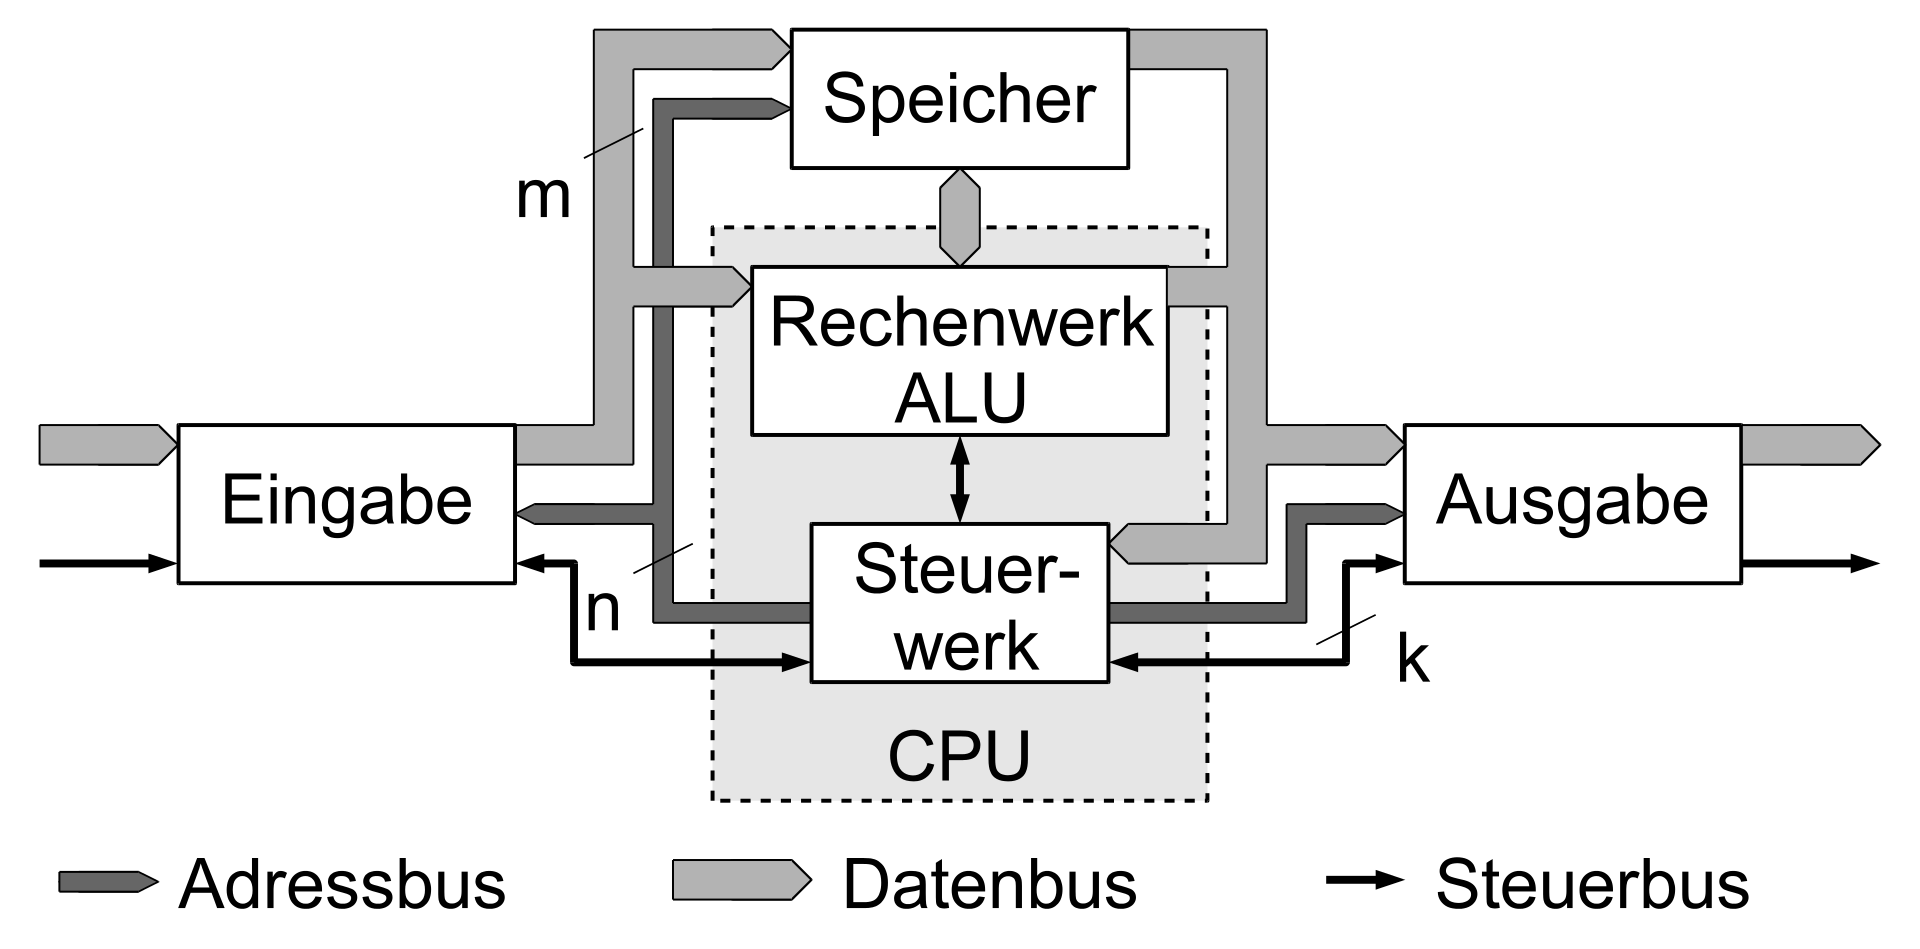
\includegraphics[scale=0.2]{img/vonneumann.png}
                        \caption[Von-Neumann-Architektur]{Von-Neumann-Architektur \cite{von-neumann-architektur}}
                        \label{fig:vonneumann}
                    \end{figure}

                \subsubsection{Harvard-Architektur}\label{lab:havard}
                    Eine weitere verbreitete Architektur ist die \textit{Harvard-Architektur}.
                    Grundlegend unterscheidet sich diese zur \textit{Von-Neumann-Architektur}
                    nur in ihrem Speicher und dem Bus. Die \textit{Harvard-Architektur} verfolgt den Ansatz,
                    Instruktionen und Daten physikalisch strikt voneinander zu trennen.
                    Dabei werden zwei separate Speicher mit eigenem Adress- sowie Datenbus verwendet.
                    Dies hat, im gegensatz zur \textit{Von-Neumann-Architektur}, den Vorteil, dass Instruktionen
                    und Daten in einem Taktzyklus gelesen bzw. geschrieben werden können. Hauptnachteil ist jedoch,
                    dass es zu Speicherfragmentierung kommt, da weder nicht genutzter Programmspeicher als Datenspeicher
                    noch umgekehrt, genutzt werden kann.
                    \\\\
                    Für den zu entwickelnden Softcore wird eine \textit{modifizierte Harvard-Architektur} verwendet, die
                    die Vorteile der beiden oben genanten Architekturen vereint. Um die Speicherfragmentierung zu eliminieren, 
                    wird wie bei der \textit{Von-Neumann-Architektur} nur ein Speicher verwendet.
                    Jedoch werden wie bei der \textit{Harvard-Architektur} zwei Bussysteme (Instruktionsbus und Datenbus)
                    implementiert. 

        \subsection{Befehlsverarbeitung}

            \subsubsection{Von-Neumann-Zyklus}
                Die Phasen der Befehlsverarbeitung werden als \textit{Von-Neumann-Zyklus}
                bezeichnet und bestehen aus folgenden fünf Teilschritten.
                Jede Phase benötigt unterschiedlich viel Zeit um sie zu durchlaufen.
                Dabei ist zu beachten, dass nicht jede Instruktion alle Phasen durchlaufen muss.
                Zum Beispiel ist ein absoluter Sprung schneller abgearbeitet als eine arithmetische
                Operation, die zunächst die Operanden aus den Registern laden,
                verarbeiten und anschließend zurück in die Register schreiben muss.
            
                \begin{description}
                    \item[Fetch] Der Befehl wird aus dem Speicher geladen.
                    \item[Decode] Der Befehl wird dekodiert und die Steuerleitungen werden gesetzt.
                    \item[Fetch Operands] Die Operanden für die ALU werden geladen 
                    \item[Execute] Das Rechenwerk verarbeitet die Operanden
                    \item[Writeback] Das Ergebnis wird in den Speicher zurück geschrieben
                \end{description}


            \subsubsection{Cycles per Instruction (CPI)}
                \textit{Cycles per Instruction (CPI)} ist ein Maß zur Beurteilung der Performanz eines Prozessors
                und sagt aus wie viele Taktzyklen benötigt werden um eine Instruktion abzuarbeiten.
                Je kleiner der CPI Wert ist desto performanter kann ein Prozessor eingeschätzt werden.
                \begin{equation}
                    CPI = \frac{Taktzyklen}{Instruktion}
                \end{equation}
                Dabei wird ein Prozessor mit einem CPI Wert größer als eins ($CPI > 1$) als subskalar,
                mit einem Wert gleich eins ($CPI = 1$) als skalar und mit einem Wert kleiner als eins
                ($CPI < 1$) als superskalarer Prozessor bezeichnet.
   

            \subsubsection{Ein-Zyklus-Prozessor}
                Als Ein-Zyklus-Prozessor wird ein Prozessor verstanden, der alle Phasen des \textit{Von-Neumann-Zyklus}
                in einem Taktzyklus abarbeitet.
                Somit ergibt sich ein CPI-Wert von eins ($CPI = 1$) und der Prozessor kann als \textit{Skalar} bezeichnet werden.
                Die maximal Taktfrequenz bzw. die minimale Taktzeit ist dabei direkt abhängig von der Signallaufzeit
                der längsten Instruktion.
                \begin{equation}
                    Taktzeit > Signallaufzeit_{Gesamtbefehl}
                \end{equation}
                Wesentlicher Vorteil dieser Architektur ist die einfache implementierung, da
                keine zusätzliche Logik benötigt wird.

            \subsubsection{Pipelining-Prozessor}
                Im gegensatz zum Ein-Zyklus-Prozessor steht der Pipelining-Prozessor.
                Statt eines gesamten Befehls wird während eines Taktzyklus nur jeweils eine Teilaufgabe abgearbeitet.
                Dabei können Teilaufgaben mehrerer Befehle gleichzeitig abgearbeitet werden.
                Eine Teilaufgabe kann dabei z.B. eine \textit{Von-Neumann-Phase} sein oder noch feiner granuliert werden.
                Da eine Teilaufgaben eine kürzere Signallaufzeit aufweist als der Gesamtbefehl,
                kann die Taktzeit kürzer sein als die Signallaufzeit des Gesamtbefehls.
                \begin{equation}
                    \begin{split}
                        Taktzeit < Signallaufzeit_{Gesamtbefehl} \\
                        Taktzeit > Signallaufzeit_{Teilaufgabe}
                    \end{split}
                \end{equation}
                Die Taktzeit ist somit nur noch abhängig von der Signallaufzeit der Teilaufgabe die am längsten dauert.
                Die Teilaufgaben eines Befehls werden auch \textit{Pipeline-Stages} genant.
                Abbildung \ref{fig:pipelining} zeigt eine vierstufige Befehlspipeline und der daraus resultierende erhöhte Gesamtdurchsatz.
                Wesentlicher Nachteil von Pipelining sind jedoch die Konflikte \textit{(Pipeline-Hazards)}
                die dabei auftreten können. Dabei können folgende drei Konfliktarten auftreten.
    
                \begin{description}
                    \item[Ressourcenkonflikte] wenn eine Stufe der Pipeline, Zugriff auf eine Ressource benötigt, die bereits von einer anderen Stufe belegt ist 
                    \item[Datenkonflikte] wenn ein Befehl, der sich in der Pipeline befindet, abhängig von einem Befehl ist, der in sich in einer der nächsten Pipelinestufen befindet
                    \item[Kontrollflusskonflikte] wenn die Pipeline abwarten muss, ob ein bedingter Sprung ausgeführt wird oder nicht
                \end{description}
                \begin{figure}[H]
                    \centering
                    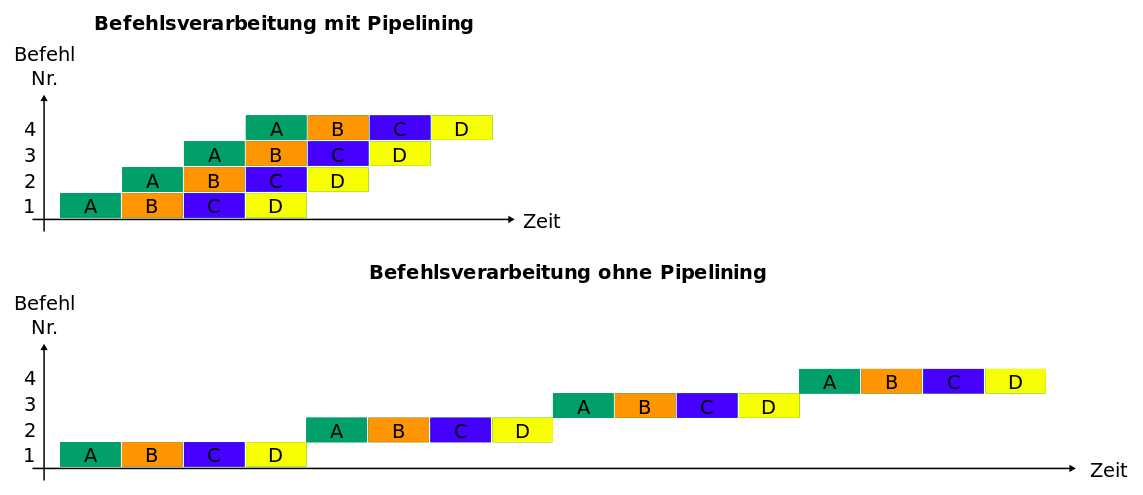
\includegraphics[scale=0.375]{img/pipelining.png}
                    \caption[Befehlsverarbeitung mit und ohne Pipelining]{Befehlsverarbeitung mit und ohne Pipelining \cite{pipelining} }
                    \label{fig:pipelining}
                \end{figure}
                \begin{description}
                    \item[A: Befehlscode laden (IF, Instruction Fetch)] 
                    \item[B: Instruktion dekodieren und laden der Daten (ID, Instruction Decoding)] 
                    \item[C: Befehl ausführen (EX, Execution)] 
                    \item[D: Ergebnisse zurückgeben (WB, Write Back)] 
                \end{description}
                Es ist jedoch zu beachten, dass Pipelining nur von Vorteil ist, wenn die Taktfrequenz, aufgrund der höheren Signallaufzeiten
                in einem Ein-Zyklus-Prozessor, nicht weiter erhöht werden kann.
                Da das gewählte \textit{FPGA}-Board nur mit $12 Mhz$ taktet, ist eine Pipelining-Architektur
                nicht von Vorteil für den Softcore, sodass eine Ein-Zyklus-Architektur gewählt werden kann um die Softcore zu implementieren.
                Dies hat zusätzlich den Vorteil, dass weniger Logikblöcke des \textit{FPGA's} benutzt werden.



        \subsection{Speicher}
                
            \subsubsection{Memory Wall}
                Als \textit{Memory Wall} bezeichnet man das wachsende Ungleichgewicht zwischen der Prozessor- und der Speichergeschwindigkeit.
                Bei frühen Computern war der Prozessor die langsamste Einheit des Rechners \cite{memory-wall}.
                Die Datenbereitstellungszeit stellte somit nur ein geringen Anteil an der Verarbeitungszeit dar.
                Seit den 1980 Jahren begann jedoch der Prozessor exponentiell schneller zu werden als der Speicher \cite{memory-cpu-gap}.
                Es kann davon ausgegangen werden dass jede fünfte Instruktion den Speicher beansprucht \cite{memory-wall}.
                Somit würde der Prozessor $20\%$ der Zeit auf Daten warten. Ein idealer Speicher würde so schnell wie der Prozessor sein
                und die Daten in einem Taktzyklus liefern.
                Wie Abbildung \ref{fig:memory-hierarchy} zeigt, wäre solch ein Speicher sehr teuer.
                Eine Maßnahme um der \textit{Memory Wall} entgegen zu wirken ist der einsatz von Cachespeicher direkt im Prozessor.
                \\\\
                Auf dem \textit{FPGA}-Board stehen die \textit{M9K}-Blöcke sowie \textit{SDRAM} als Speicher zu Verfügung (Siehe \ref{lab:hardware}).
                Dabei wir der \textit{SDRAM} über eine 16 Bit Interface angesprochen. Der \textit{RV32I} Befehlssatz ist jedoch 32 Bit breit.
                Dadurch werden zwei Taktzyklen benötigt um eine Instruktion aus dem Speicher zu laden und würde dadurch den Softcore ausbremsen.
                Um das Problem der \textit{Memory Wall} zu lösen werden die \textit{M9K}-Blocke des \textit{FPGA's} als Speicher benutzt.
                Diese können in der Breite frei variiert werden und ermöglichen den Zugriff auf die Daten in einem Taktzyklus.
                Wesentlicher Nachteil dieser Lösung ist, dass nur \textit{67584B} Speicher für Daten und Instruktionen zu Verfügung stehen.
                
                \begin{figure}[H]
                    \centering
                    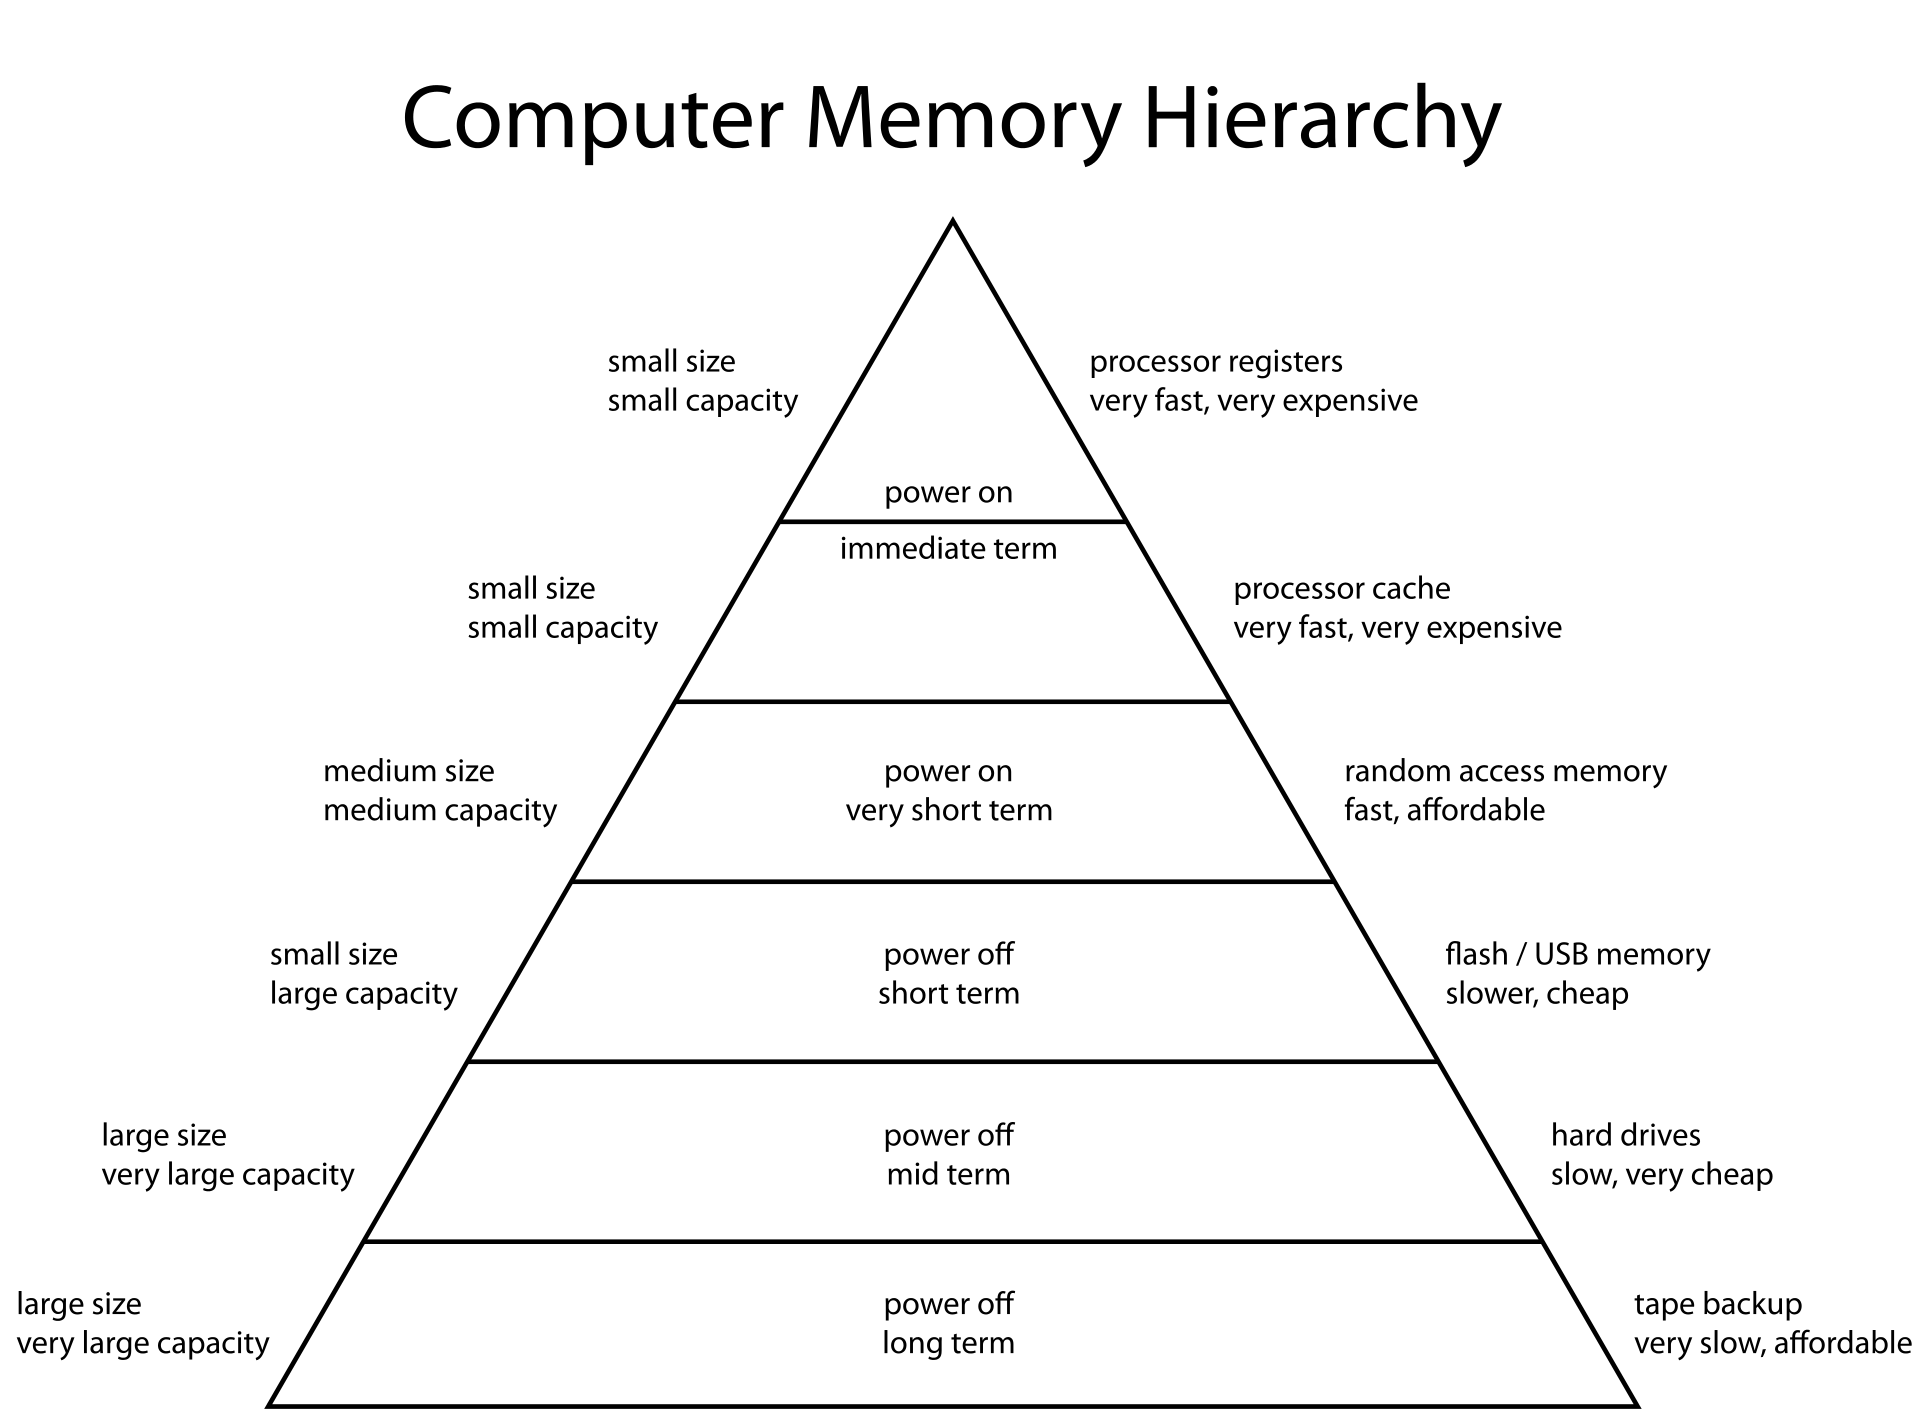
\includegraphics[scale=0.2]{img/speicherpyramide.png}
                    \caption[Speicherpyramide]{Speicherpyramide \cite{memory-hierarchy}}
                    \label{fig:memory-hierarchy}
                \end{figure}


            \subsubsection{Speicherausrichtung}\label{lab:mem-order}
                Da eine \textit{modifizierte Harvard-Architektur} gewählt wurde (Siehe \ref{lab:havard}), liegen im Speicher
                sowohl Daten als auch Instruktionen. Die Instruktionen sind hierbei in vier Byte Grenzen zu halten
                (natürliche Ausrichtung) \cite{riscv-isa-specs}[2.2].
                Der Befehlssatz lässt es jedoch der EEI (Siehe \ref{lab:eei}) überlassen, ob die Daten auch natürlich ausgerichtet liegen sollen
                \cite{riscv-isa-specs}[2.6].
                Der Vorteil von natürlich ausgerichteten Daten liegt darin, das keine zusätzliche Logik benötigt wird um Daten im Speicher
                auszulesen bzw. zu schreiben. Wesentlicher Nachteil ist die Speicherfragmentierung, da im Worst-case 32 Bit für einen 8 Bit 
                Wert verbraucht werden. Die ungenutzten 24 Bit $(32 Bit - 8 Bit = 24 Bit)$ werden mit Nullen aufgefüllt.
                Der Einfachheit halber wird der Ansatz des natürlich ausgerichteten Speichers gewählt.

                





                
            
                
            
           
            
            

            

            



            
    
        

    
